\chapter{Contexte et Motivation}

\paragraph{}
Dans le domaine des communications réseaux pair à pair, il est nécessaire d'établir une communication directe entre deux clients. Cependant, certains défis se 
posent lors de la mise en place d'une telle communication, notamment en présence de dispositifs de traduction d'adresses réseau (NAT pour "Network address translation") 
qui limitent la connectivité directe entre les clients.


\section{Les dispositifs de traduction d'adresses réseau (NAT)}

\paragraph{}
Le NAT est souvent utilisé dans les réseaux domestiques et les petites entreprises pour partager une seule adresse IP publique fournie par le fournisseur d'accès à Internet (FAI) entre plusieurs dispositifs du réseau local. 
Plutôt que d'attribuer une adresse IP publique unique à chaque dispositif, le NAT attribue des adresses IP privées à chaque dispositif du réseau local. Lorsque ces dispositifs se connectent à Internet, le NAT traduit 
automatiquement les adresses IP privées en adresse IP publique, permettant ainsi à ces dispositifs de communiquer avec des serveurs sur Internet.

\paragraph{}
Outre la conservation des adresses IP publiques, le NAT offre également une certaine forme de sécurité en masquant les adresses IP privées des dispositifs internes. Cela rend plus difficile pour les personnes 
extérieures au réseau local de cibler directement ces dispositifs.

\newpage
\paragraph{}
Cependant, le NAT introduit une limitation en ce qui concerne la connectivité entre les dispositifs du réseau local et les dispositifs externes. Étant donné que les adresses IP privées ne sont pas routables sur Internet, 
les dispositifs internes d'un réseau NAT ne peuvent pas recevoir de connexions entrantes directement. Ils sont uniquement capables d'initier des connexions sortantes vers des serveurs externes. Cela signifie que les dispositifs 
internes ne peuvent pas être facilement accessibles depuis Internet, sauf si des règles spécifiques de translation de port (port forwarding) sont configurées pour rediriger les connexions entrantes vers des dispositifs spécifiques.

\paragraph{}
En résumé, le NAT offre une solution efficace pour partager une adresse IP publique et protéger les dispositifs internes, mais il peut limiter la connectivité directe entre les clients du réseau local et les dispositifs externes.


\begin{figure}[h]
\centering
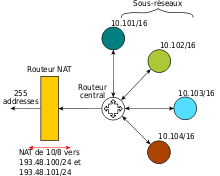
\includegraphics[width=0.8\textwidth]{assets/nat.png}
\caption{Exemple de NAT}
\end{figure}

\newpage

\section{Problèmes liés aux dispositifs de traduction d'adresses réseau (NAT)}

\paragraph{}
Les dispositifs de traduction d'adresses réseau (NAT) sont couramment utilisés pour partager une seule adresse IP publique entre plusieurs appareils d'un réseau local. Les NAT 
peuvent être trouvés dans de nombreux environnements, tels que les réseaux domestiques, les réseaux d'entreprises et même les réseaux mobiles.

\paragraph{}
Lorsqu'un client se trouve derrière un NAT, il reçoit une adresse IP privée non routable, qui n'est pas accessible depuis Internet. Cela rend difficile l'établissement 
d'une communication directe avec d'autres clients qui se trouvent également derrière des NAT.

\section{La nécessité d'un tiers pour faciliter l'établissement de la connexion}

\paragraph{}
Dans le contexte des communications pair à pair, il devient nécessaire d'avoir un tiers (un serveur intermédiaire) pour faciliter l'établissement de la connexion entre les clients.
Ce tiers agit comme un relai en permettant aux clients de s'échanger les informations nécessaires pour établir la connexion, même s'ils ne peuvent pas le faire directement en raison des NAT.

\paragraph{}
Le relai joue un rôle crucial en tant qu'entremetteur dans le processus d'établissement de la connexion entre les clients. Lorsqu'un client souhaite établir une communication avec un autre client,
il s'enregistre auprès du relai et fournit des informations telles que son adresse IP publique et son port. Le relai enregistre ces informations et les rend disponibles aux autres clients qui souhaitent
se connecter à ce client spécifique.

\paragraph{}
Lorsqu'un client souhaite établir une connexion avec un autre client, il contacte le relai pour obtenir les informations de connexion de sa cible. Le relai transmet alors ces informations au client
demandeur, lui permettant ainsi d'établir une connexion directe avec le client cible.

\paragraph{}
Il est important de noter que le rôle du relai se limite à faciliter l'établissement de la connexion en transmettant les informations nécessaires entre les clients. Une fois que la connexion directe
est établie entre les clients, les données échangées ne passent pas par le relai, mais sont directement transmises entre les clients.

\section{Solutions alternatives ou complémentaires pour contourner les limitations des dispositifs NAT}

\paragraph{}
Bien que les dispositifs de traduction d'adresses réseau (NAT) puissent poser des défis en matière de connectivité directe entre les clients, il existe plusieurs solutions alternatives ou complémentaires pour contourner ces limitations. En voici quelques-unes :

\paragraph{Les protocoles TURN et STUN}

\paragraph{}
Le protocole STUN permet à un client d'obtenir des informations sur son adresse IP publique et le type de NAT qu'il traverse. Cela permet au client de comprendre comment il est connecté au réseau et d'adapter ses stratégies de 
connexion en conséquence. STUN est généralement utilisé pour faciliter l'établissement de connexions pair à pair lorsque les clients sont derrière des NAT symétriques ou des pare-feu restrictifs.

\paragraph{}
Le protocole TURN est utilisé lorsque les connexions directes ne sont pas possibles en raison de pare-feu ou de NAT restrictifs. TURN utilise un serveur intermédiaire (relais) auquel les clients se connectent pour acheminer 
leurs données. Ce serveur intermédiaire agit comme un proxy et transfère les données entre les clients. Cela permet aux clients de communiquer même s'ils ne peuvent pas établir une connexion directe.

\paragraph{}
Lorsqu'un client rencontre des difficultés pour établir une connexion directe en raison des restrictions du réseau, il peut utiliser STUN pour obtenir son adresse IP publique, puis essayer d'établir une connexion directe. 
Si cela échoue, le client peut passer à l'utilisation de TURN pour acheminer les données via un serveur relais.

\paragraph{}
Il est important de noter que l'utilisation de TURN peut entraîner une latence supplémentaire car les données doivent être acheminées via le serveur relais. De plus, l'utilisation d'un serveur relais peut entraîner des coûts supplémentaires, 
notamment si vous utilisez un service cloud ou un fournisseur tiers pour héberger le serveur.
